\section{Applications and Evaluation}
\label{sec:eval}

We have implemented the interpolation algorithm in a modified version of the \dReal SMT solver.\footnote{Currently available in the branch \url{https://github.com/dzufferey/dreal3/}.} %\footnote{Once the implementation is stable, the interpolation will be merged into the main repository of \dReal}.
The proofs produced by \dReal can be very large, i.e., gigabytes.
Therefore, the interpolants are built and simplified on-the-fly.
The full proof is not kept in memory.
We modified the ICP loop and the contractors which are responsible for the pruning steps.
The overhead induced by the interpolant generation over the solving time is smaller than 10\%.

The ICP loop (Figure~\ref{icpalgo}) builds a proof starting from the root of the proof tree and exploring the tree like a depth-first search.
On the other hand, the interpolation rules build the interpolant starting from the proof's leaves.
Our implementation modifies the ICP loop to keep a stack $P$ of partial interpolants alongside the stack of branching points $S$.
When branching (line~\ref{code:branch}), the value used to split $\vec D_1$ and $\vec D_2$ is pushed on $P$.
The pruning steps (line~\ref{code:prune2}) are converted to a proof as shown in Figure~\ref{fig:prune}.
When a contradiction is found (line~\ref{code:prune1}), $P$ is popped to the branching point where the search resumes and the corresponding partial interpolant is pushed back on $P$.
When the ICP loop ends, $P$ contains the final interpolant.

\paragraph{Interpolant sizes.}
The ICP algorithm implemented in \dReal eagerly prunes the domain by applying repeatedly \emph{all} the constraints.
Therefore, it usually generates large proofs often involving all the constraints and all the variables.
Interpolation can extract more precise information from the proof.
Intuitively, an interpolant which is much smaller than the proof are more likely to be useful in practice.
In this test, we try to compare the size of the proof against the size of the interpolants using benchmark from the Flyspeck project~\cite{2015arXiv150102155H}, certificates for Lyapunov functions in powertrain control systems~\cite{DBLP:conf/hybrid/KapinskiDSA14} and the other examples presented in the rest of this section.

%The Flyspeck project has built a mechanized proof of the Kepler conjecture.
%Part of the proof requires showing the unsatisfiability of nonlinear formulas.
%In previous work~\cite{DBLP:conf/synasc/GaoKC14}, part of these formulas were translated to the input format of \dReal.
%\todo[inline]{Toyota}

We run \dReal with a 20 minutes timeout and generate 1063 interpolants.
Out of these, 501 are nontrivial.
In Figure~\ref{fig:flyspeck} we plot the number of inequalities in the nontrivial interpolants against the size of the proof without the \weaken steps.
For similar proofs, we see that the interpolants can be order of magnitude simpler than the proofs and other interpolants obtained by different partitions of the formula.
The trivial interpolants still bring information as they mean that the only one side is part of the unsatisfiable core.


\begin{figure}
\centering
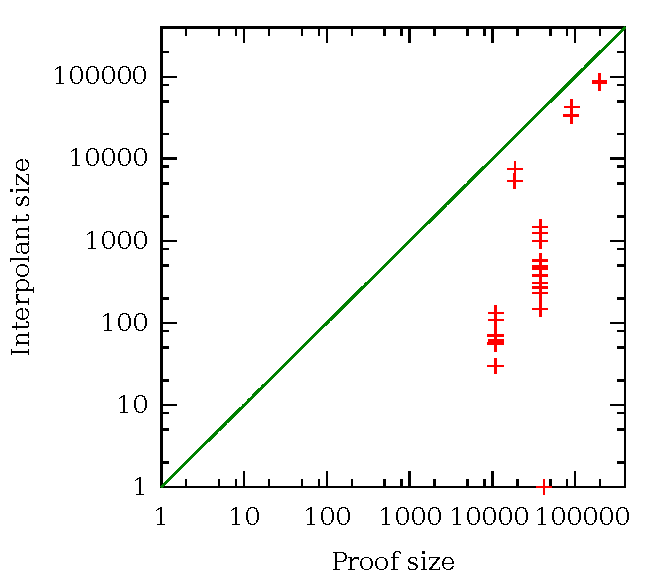
\includegraphics[scale=0.6]{img/itpsize2.pdf}
\caption{Size of the interpolants (number of inequalities) compared to the size of the proof.}
\label{fig:flyspeck}
\end{figure}


\paragraph{Hybrid system verification.}
Our method can compute interpolants for systems of ODEs.
For instance, we can check that two trajectories do not intersect.
Figure~\ref{fig:ode} shows an interpolant obtained for the following equations:
\begin{eqnarray*}
A: &~~~~&  x_t = x₀ + \int_0^t \! -x + cos(x) \, \mathrm{d}x ∧ x₀ = 3 ∧ 0 ≤ t ≤ 2 \\
B: &~~~~&  y_t = y₀ + \int_0^t \! -y + sin(y-1) \, \mathrm{d}y ∧ y₀ = 2 ∧ x_t = y_t
\end{eqnarray*}

A large portion, 479 out of 1063, of our examples involves differential equations.
These examples include:
airplane control~\cite{Bae201513},
bouncing balls, networked water tanks,
models of cardiac cells~\cite{DBLP:conf/cmsb/LiuKGZC14},
verification of the trajectory planning and tracking stacks of autonomous vehicle (in particular, for lane change maneuver~\cite{althoff2014online}),
and example from \dReal regression tests.
Table~\ref{tbl:ode} shows statistics about the interpolants for each family of examples.
% apex_0_0_unsat

\begin{table}
\centering
\begin{tabular}{l|cccrrr}
Family            & \#tests    & ~\#flow &  ~\#var  & proof size      & ~interpolant size & time \\
\hline
Airplane control  &       53   &  [1,4] & [56,61] & [4213,24249]    &  [70,10260]     &   [57s,178s]  \\
Apex              &       17   &   1    &  44     &          23     &  [0,22]         &    [5s,9s]    \\
Bouncing ball     &      165   &   2    &  128    &         857     &  [0,28]         &  [1.6s,5.5s]  \\
Cardiac cells     &       37   &   4    &  71     &          15     &  [0,1]          & ~[15m,20m]    \\
Water tanks       &       68   &  [4,8] & [18,30] & [6530,225099]   &  [331,92594]    &  [7s,12m]     \\
Lane change       &       15   &   1    &  44     &          24     &  [0,23]         &   [19s,20s]   \\
Other tests       &      142   &   1    &  5      &           2     &  [0,1]          &  [0.1s,1s]   
\end{tabular}

\vspace{1ex}

\caption{
    Results for the interpolation of ODEs.
    The [\_,\_] notation stands for intervals that cover the values for the whole families of examples.
    The first column indicates the family.
    The next three columns contains the number of tests in the family, the number of flows and variables in the tests.
    The last three columns shows the size of the proofs, interpolants, and the solving time.
}
\label{tbl:ode}
\end{table}

\paragraph{Robotic design.}
Often, hybrid system verification is used in model-based design.
An expert produces a model of the system which is then analysed.
However, it is also possible to extract models directly from the manufacturing designs.
As part of an ongoing project about co-design of both the software and hardware component of robots~\cite{react}, we extract equations from robotic designs.
In the extracted models, each structural element is represented by a 3D vector for its position and a unit quaternion for the orientation.
The dimension of the elements and the joints connecting them corresponds to equations that relate the position and orientation variables.
Active elements, such as motors, also have specific equations associated to them.

This approach provides models faithful to the actual robots, but it has the downside of producing large systems of equations.
To verify such systems, we need to simplify them.
Due to the presence of trigonometric functions we cannot use quantifier elimination for polynomial systems of equations~\cite{qepcad}.
However, we use interpolation as an approximation of quantifier elimination.

Let us consider a kinematic model, $𝓚(\vec x,\vec y,\vec z)$ where $\vec x$ is a set of design and input parameters, $\vec y$ is the variables that represent the state of each component of the robot, and $\vec z$ is the variables that represent the parts of the state needed to prove the property of interest.
For instance, in the case of a robotic manipulator, $\vec x$ contain the sizes of each element and the angles of the servo motors and $\vec z$ is the position of the effector.
$\vec y$ is determined by the designed of the manipulator.

Fully controlled systems have the property that once the design and input parameters are fixed, there is a unique solution for remaining variables in the model.
Therefore, we can create an interpolation query:
\begin{eqnarray*}
A: &~~~~ &  𝓚(\vec x,\vec y,\vec z) ∧ \\
B: &~~~~ &  𝓚(\vec x,\vec v,\vec w) ∧ (\vec z-\vec w)² ≥ ε² \quad \text{where} ~ ε > δ
\end{eqnarray*}
$\vec y, \vec v$ are two copies of the variables we want to eliminate.
Since the kinematic is a function of $\vec x$ which is the same for the two copies $\vec z$ and $\vec w$ should be equal.
Therefore, the formula we build has no solution and we get an interpolant $I(\vec x,\vec z)$ which is an ε-approximation of $∃ \vec y.\,𝓚(\vec x,\vec y,\vec z)$.

\begin{figure}
\begin{subfigure}{0.45\textwidth}
  \centering
  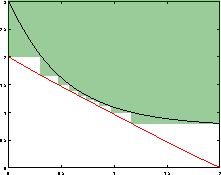
\includegraphics[scale=1.5]{img/ode.pdf}
  \caption{ Interpolant for system of nonlinear ODEs. 
            The black and red curves are the trajectories described by $A$ and $B$.
            The green area is the interpolant.
            }
  \label{fig:ode}
\end{subfigure}
\hfill
\begin{subfigure}{0.5\textwidth}
  \centering
  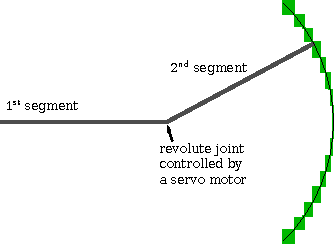
\includegraphics[scale=1]{img/arm.pdf}
  \caption{
    Model of a 1-DOF robotic manipulator composed of two 100mm long segments.
    The black line shows the effector's reach and the green cubes are the approximation obtained by interpolation where ε is 10mm.
  }
  \label{fig:robot}
\end{subfigure}
\caption{Application of interpolation to nonlinear systems}
\end{figure}


\begin{example}
Consider the simple robotic manipulator show in Figure~\ref{fig:robot}.
The manipulator has one degree of freedom.
It is composed of two beams connected by a revolute joint controlled by a servo motor.
The first beam is fixed.

The original system of equations describing this system has 22 variables: 7 for each beam, 7 for the effector, and 1 for the revolute joint.
Using the interpolation we obtain a simpler formula with only 4 variables: 3 for the effector's position and 1 for the joint.
Table~\ref{tbl:robot} shows some statistics about the interpolants we obtained using different ε for a one and a two degrees of freedom manipulators.

\begin{table}
\centering
\begin{tabular}{l|clrr}
1-DOF Model & ~ \#var  ~~ & Theory   & \#th.~atoms & ~~ time \\
\hline
\hline
original & 22 & polynomial deg.~2, trig.~fct.   & 24    & - \\
\hline
ε = 10   & 4  & linear                          & 1073  & 0.3s \\
ε = 5    & 4  & linear                          & 2757  & 0.6s \\
ε = 3    & 4  & linear                          & 3307  & 0.8s \\
ε = 2    & 4  & linear                          & 6137  & 1.3s \\
ε = 1    & 4  & linear                          & 12485 & 2.6s \\
\end{tabular}

\vspace{2ex}

\begin{tabular}{l|clrr}
2-DOF Model    & ~ \#var  ~~ & Theory   & \#th.~atoms & ~~ time \\
\hline
\hline
original & 30 & polynomial deg.~2, trig.~fct.   & 32        & - \\
\hline
ε = 10   & 5  & linear                          & 45686     & 2m\,7s \\
ε = 7    & 5  & linear                          & 97068     & 3m\,51s  \\
ε = 5    & 5  & linear                          & 184762    & 6m\,41s  \\
ε = 3    & 5  & linear                          & 547558    & 19m\,4s  \\
ε = 2    & 5  & linear                          & 1151454   & 41m\,51s  \\
\end{tabular}

\vspace{1ex}

\caption{
    Comparison of the original model of a 1 and 2 degrees of freedom manipulator against approximations obtained using interpolation.
    For the size of the formulas we report the number of theory atoms in the formula.
    The last column shows the time \dReal takes to compute the interpolants.
}
\label{tbl:robot}
\end{table}


\end{example}





